\documentclass[prl,twocolumn,superscriptaddress,floatfix]{revtex4}
\usepackage[utf8]{inputenc}
\usepackage{graphicx}
\usepackage{float}
\usepackage{amsmath,amssymb,amstext}

% get rid of hbox badness 10000 in bbl file
\usepackage{etoolbox}
\apptocmd{\sloppy}{\hbadness 10000\relax}{}{}

\begin{document}

\title{Analysis of the Fourier Transformation and its Applications}
\author{Junseo Shin}
\affiliation{Department of Physics, Washington University, St.\ Louis, Missouri 63130}
\author{Jeremy Smith}
\affiliation{Department of Physics, Washington University, St.\ Louis, Missouri 63130}

\date{\today}

\begin{abstract}
The Fourier Transform converts a signal---e.g. AC current and radio waves---intially presented in the time domain into the frequency domain.
Decomposing a signal into its constituent frequencies allows more information content to be extracted from a signal 
thus the Fourier Transform became a powerful tool in signal processing and analysis. [SEC 1]

Modern technology, such as the Stanford Research Systems SR770, utilizes the Fast Fourier Transform (FFT);
a numerical algorithm that computes the Discrete Fourier Transform (DFT) of a sequence (or continuous signal) in rapid time--- i.e. reducing the computational complexity of a time series from $O(n^2)$ to $O(n \log n)$\cite{FFT}. [SENTENCE 2]
Although FFT allows for extremely fast and efficient frequency domain representation, there are limitations regarding the resolution of the frequency domain,
its sensitivity to noise, and spectral leakage. [SEC 3?]

Here we show how FFT can be used for finding signal amongst noise, tuning into AM radio, and identifying properties of the fluxgate magnometer. [SEC 4]

Fourier Transformations present a new set of tools for understanding how a signal behaves in the frequency domain.
We deciphered information contained in a particular signal by utilitizing spectral density, harmonic analysis, and a rf (radio frequency) receiver module . [SEC 5]

From the three experiments, the paradigm of analysis was rendered impossible in the time domain, but is now possible in the frequency domain.[SEC 6]

We prospect that these experimental explorations will capture the utility and importance of Fourier methods in signal processing and analysis.
Furthermorem, an intuitive understanding of Fourier Transformations will reveal the hidden yet visible applications of Fourier methods in the modern world. [SEC 7]
\end{abstract}
\maketitle

Famous mathmetician and educator Gilbert Strang stated that the FFT is "the most important numerical algorithm of our lifetime"\cite{strang}.
This was in 1994 before the invention of the Iphone, and only a year after the World Wide Web was released into public domain\cite{cernweb}.
Now every handheld device utilizes a Fourier Transform in some fashion, from the cellular networks \& WiFi signals that connect us to the internet to the software that processes the images we take. But first we should understand what a Fourier Transform before we can understand its applications:

The Fourier Transform is an integral transform that takes the time series of a function/signal and ouputs a function of frequency. For the math inclined, it is simply
\begin{equation}
f(\xi) = \int_{-\infty}^{\infty} f(x)e^{-i2\pi \xi x}  \label{firstequation}
\end{equation}
From this it becomes clear that for frequencies with associated harmonics, the integral product will be greater than zero, whereas those without will collapse to zero.
Even more importantly is in our new function the product determined for each frequency is proportional to the strength of its harmonic within the Fourier Series.
This can be best visualized using an oscilloscope (TDS1012) which displays data in the time domain and a Stanford Research spectrum analyzer 770 (SR770) which displays the frequency domain.
Also, note that the SR770 uses FFT which splices the time series into discrete segments and efficiently computes the DCT at blazing speeds. These tools as well as a function generator and electronic modules provided
by Teach Spin are the main tools used in our exploration of the Fourier Transform.

\begin{figure}[H]
    \begin{center}
    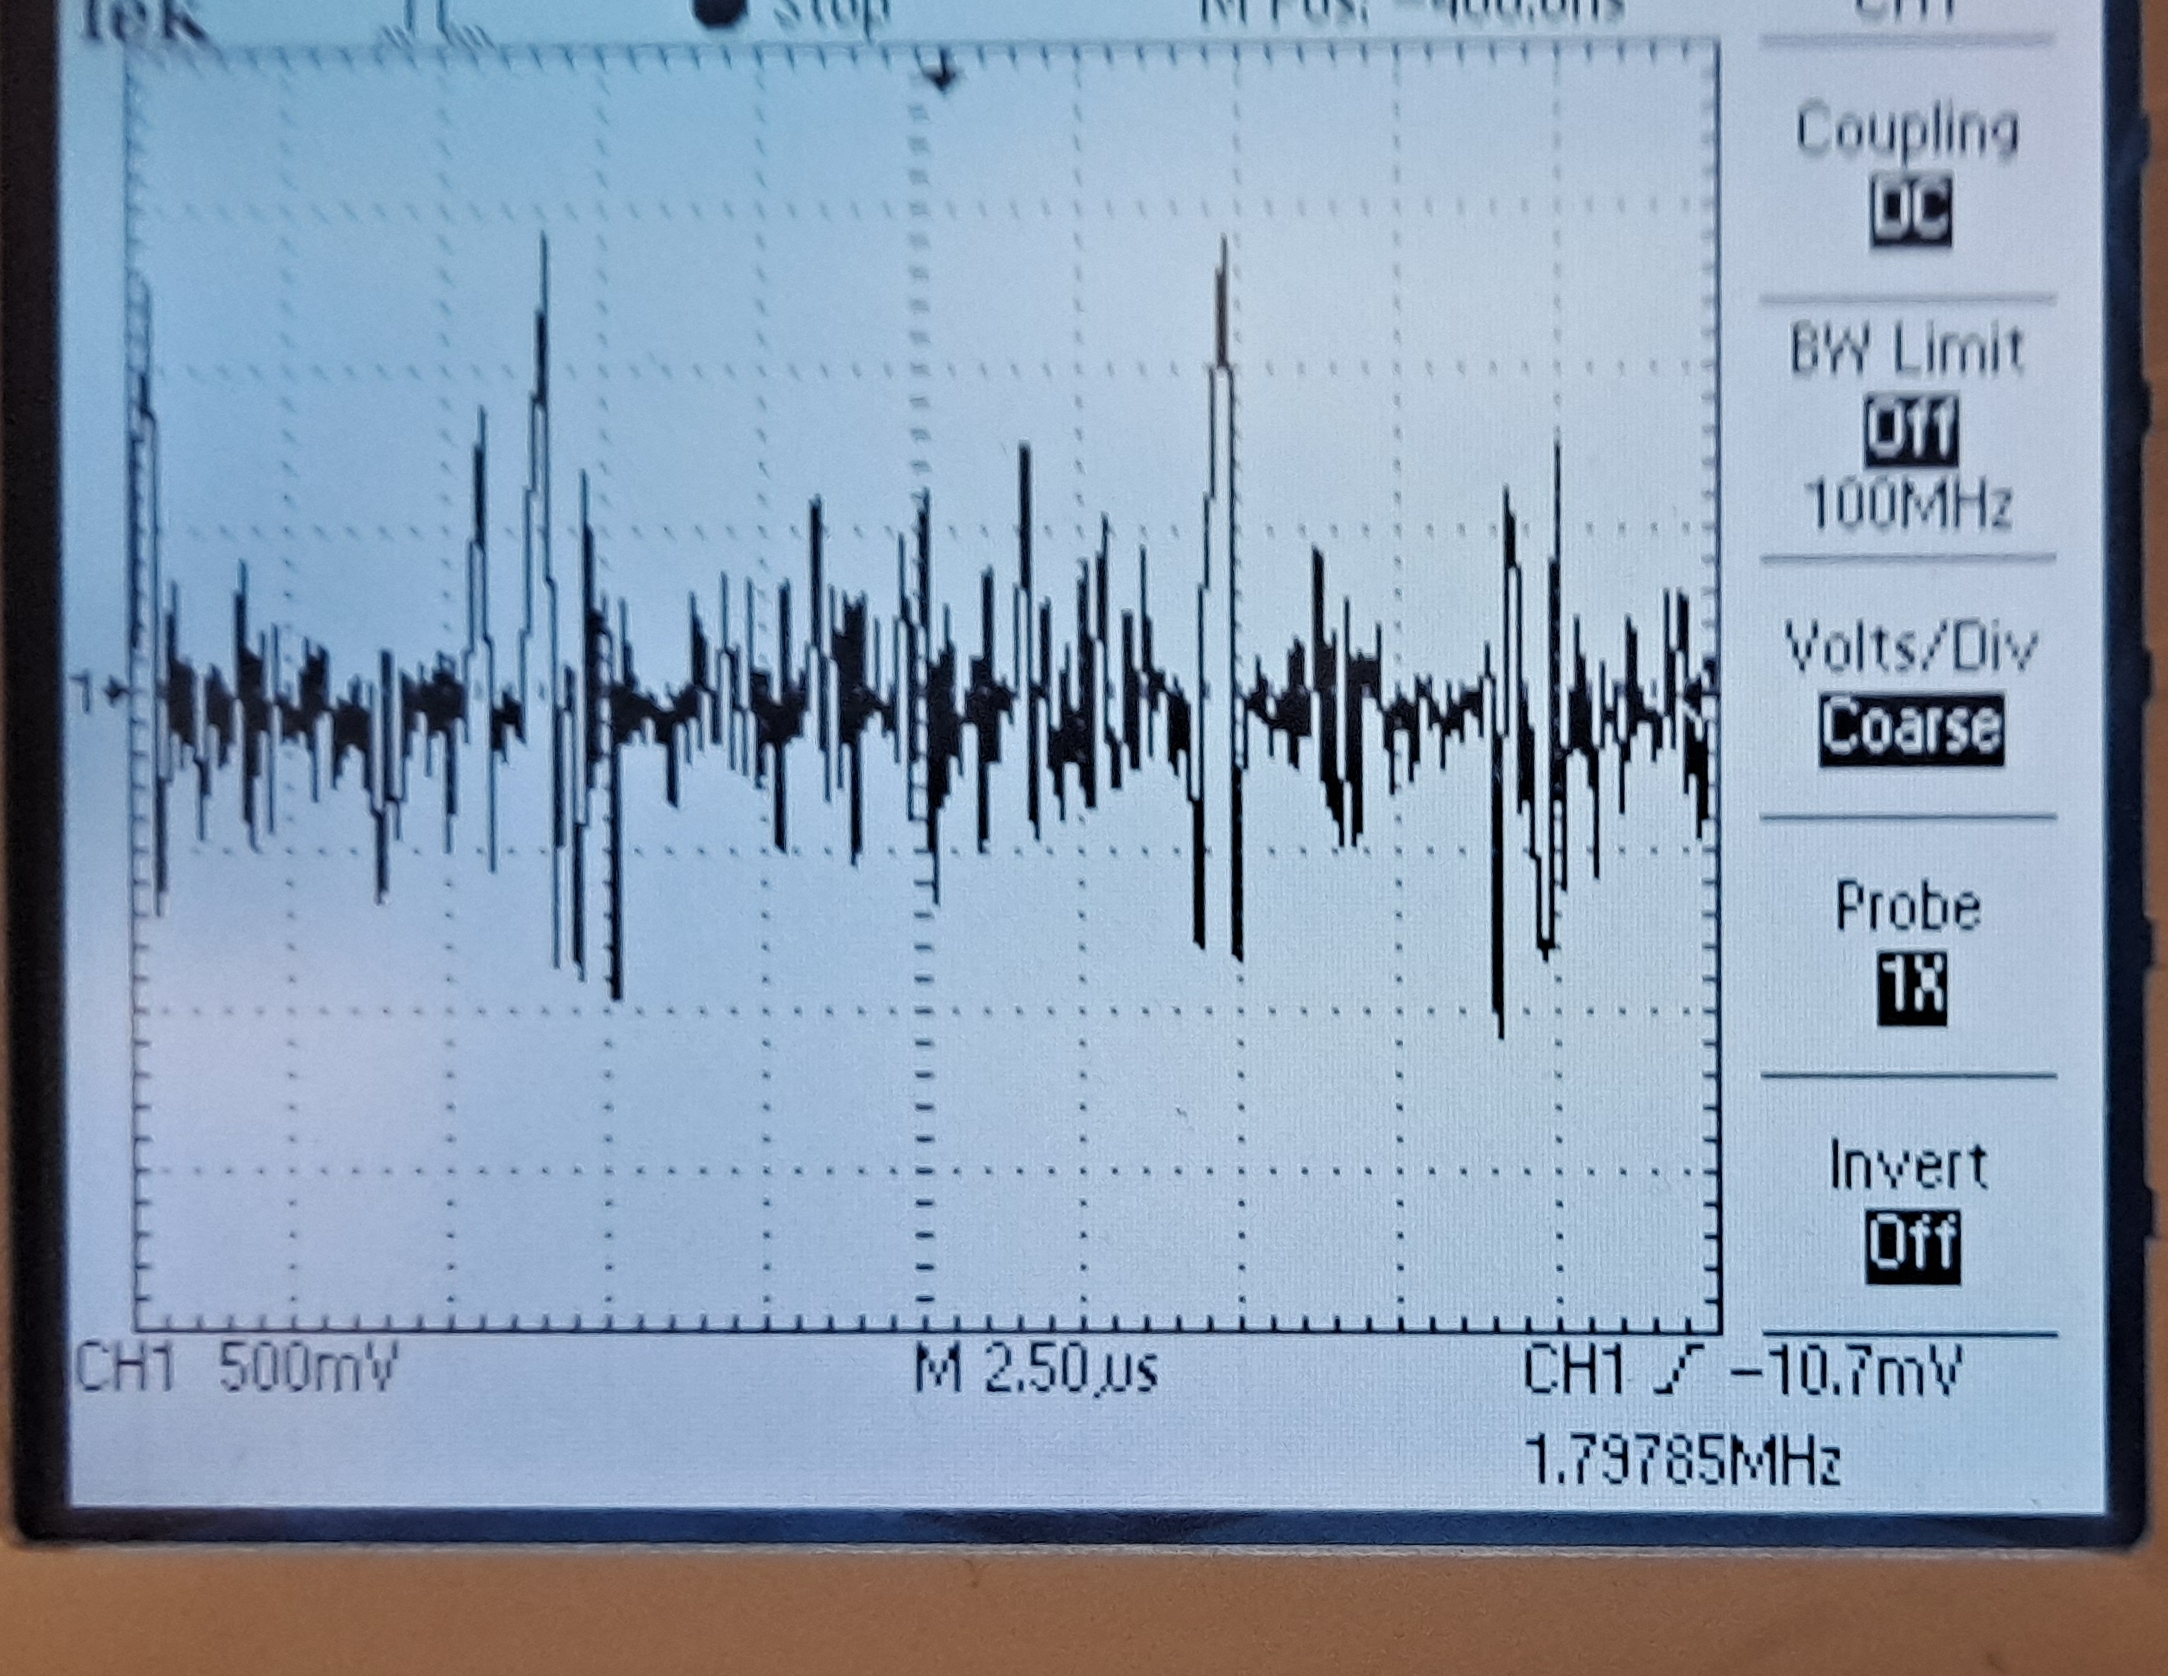
\includegraphics[width = 0.3\textwidth]{Time Data.jpg}
    \includegraphics[width = 0.3\textwidth]{Basic Sinusodial.jpg}
    \caption{\label{fig:1}Oscilloscope (top) and Spectrum (bottom) view for a 50 kHz, 5 V sine wave superimposed with noise}
    \end{center}
\end{figure}
For our first experiment we analyzed an unknown signal hidden under noise. Initially, as a proof of concept, we had a small amount of noise applied to a distinct strong signal.
As shown in Fig. \ref{fig:1}, using the time domain approach (scope) demonstrates an interesting but indecipherable signal.
In the partnering image is the SR770 display in which it is almost impossible to miss the pure sinusoidal. 
We can also read the power of that individual signal itself. Due to the product of $f(x)$ and $e^{-i2 \pi \xi x}$, each frequency in the spectrum is displayed in a way that is proportional to its power.


One could, theoretically and with great difficulty, examine the time domain signal and derive the pure sinusodial, but
becomes exceptionally difficult for a signal under much heavier noise as shown in Fig. \ref{fig:2}. 

\begin{figure}[H]
    \begin{center}
    \includegraphics[width = 0.3\textwidth]{Time Data C.jpg}
    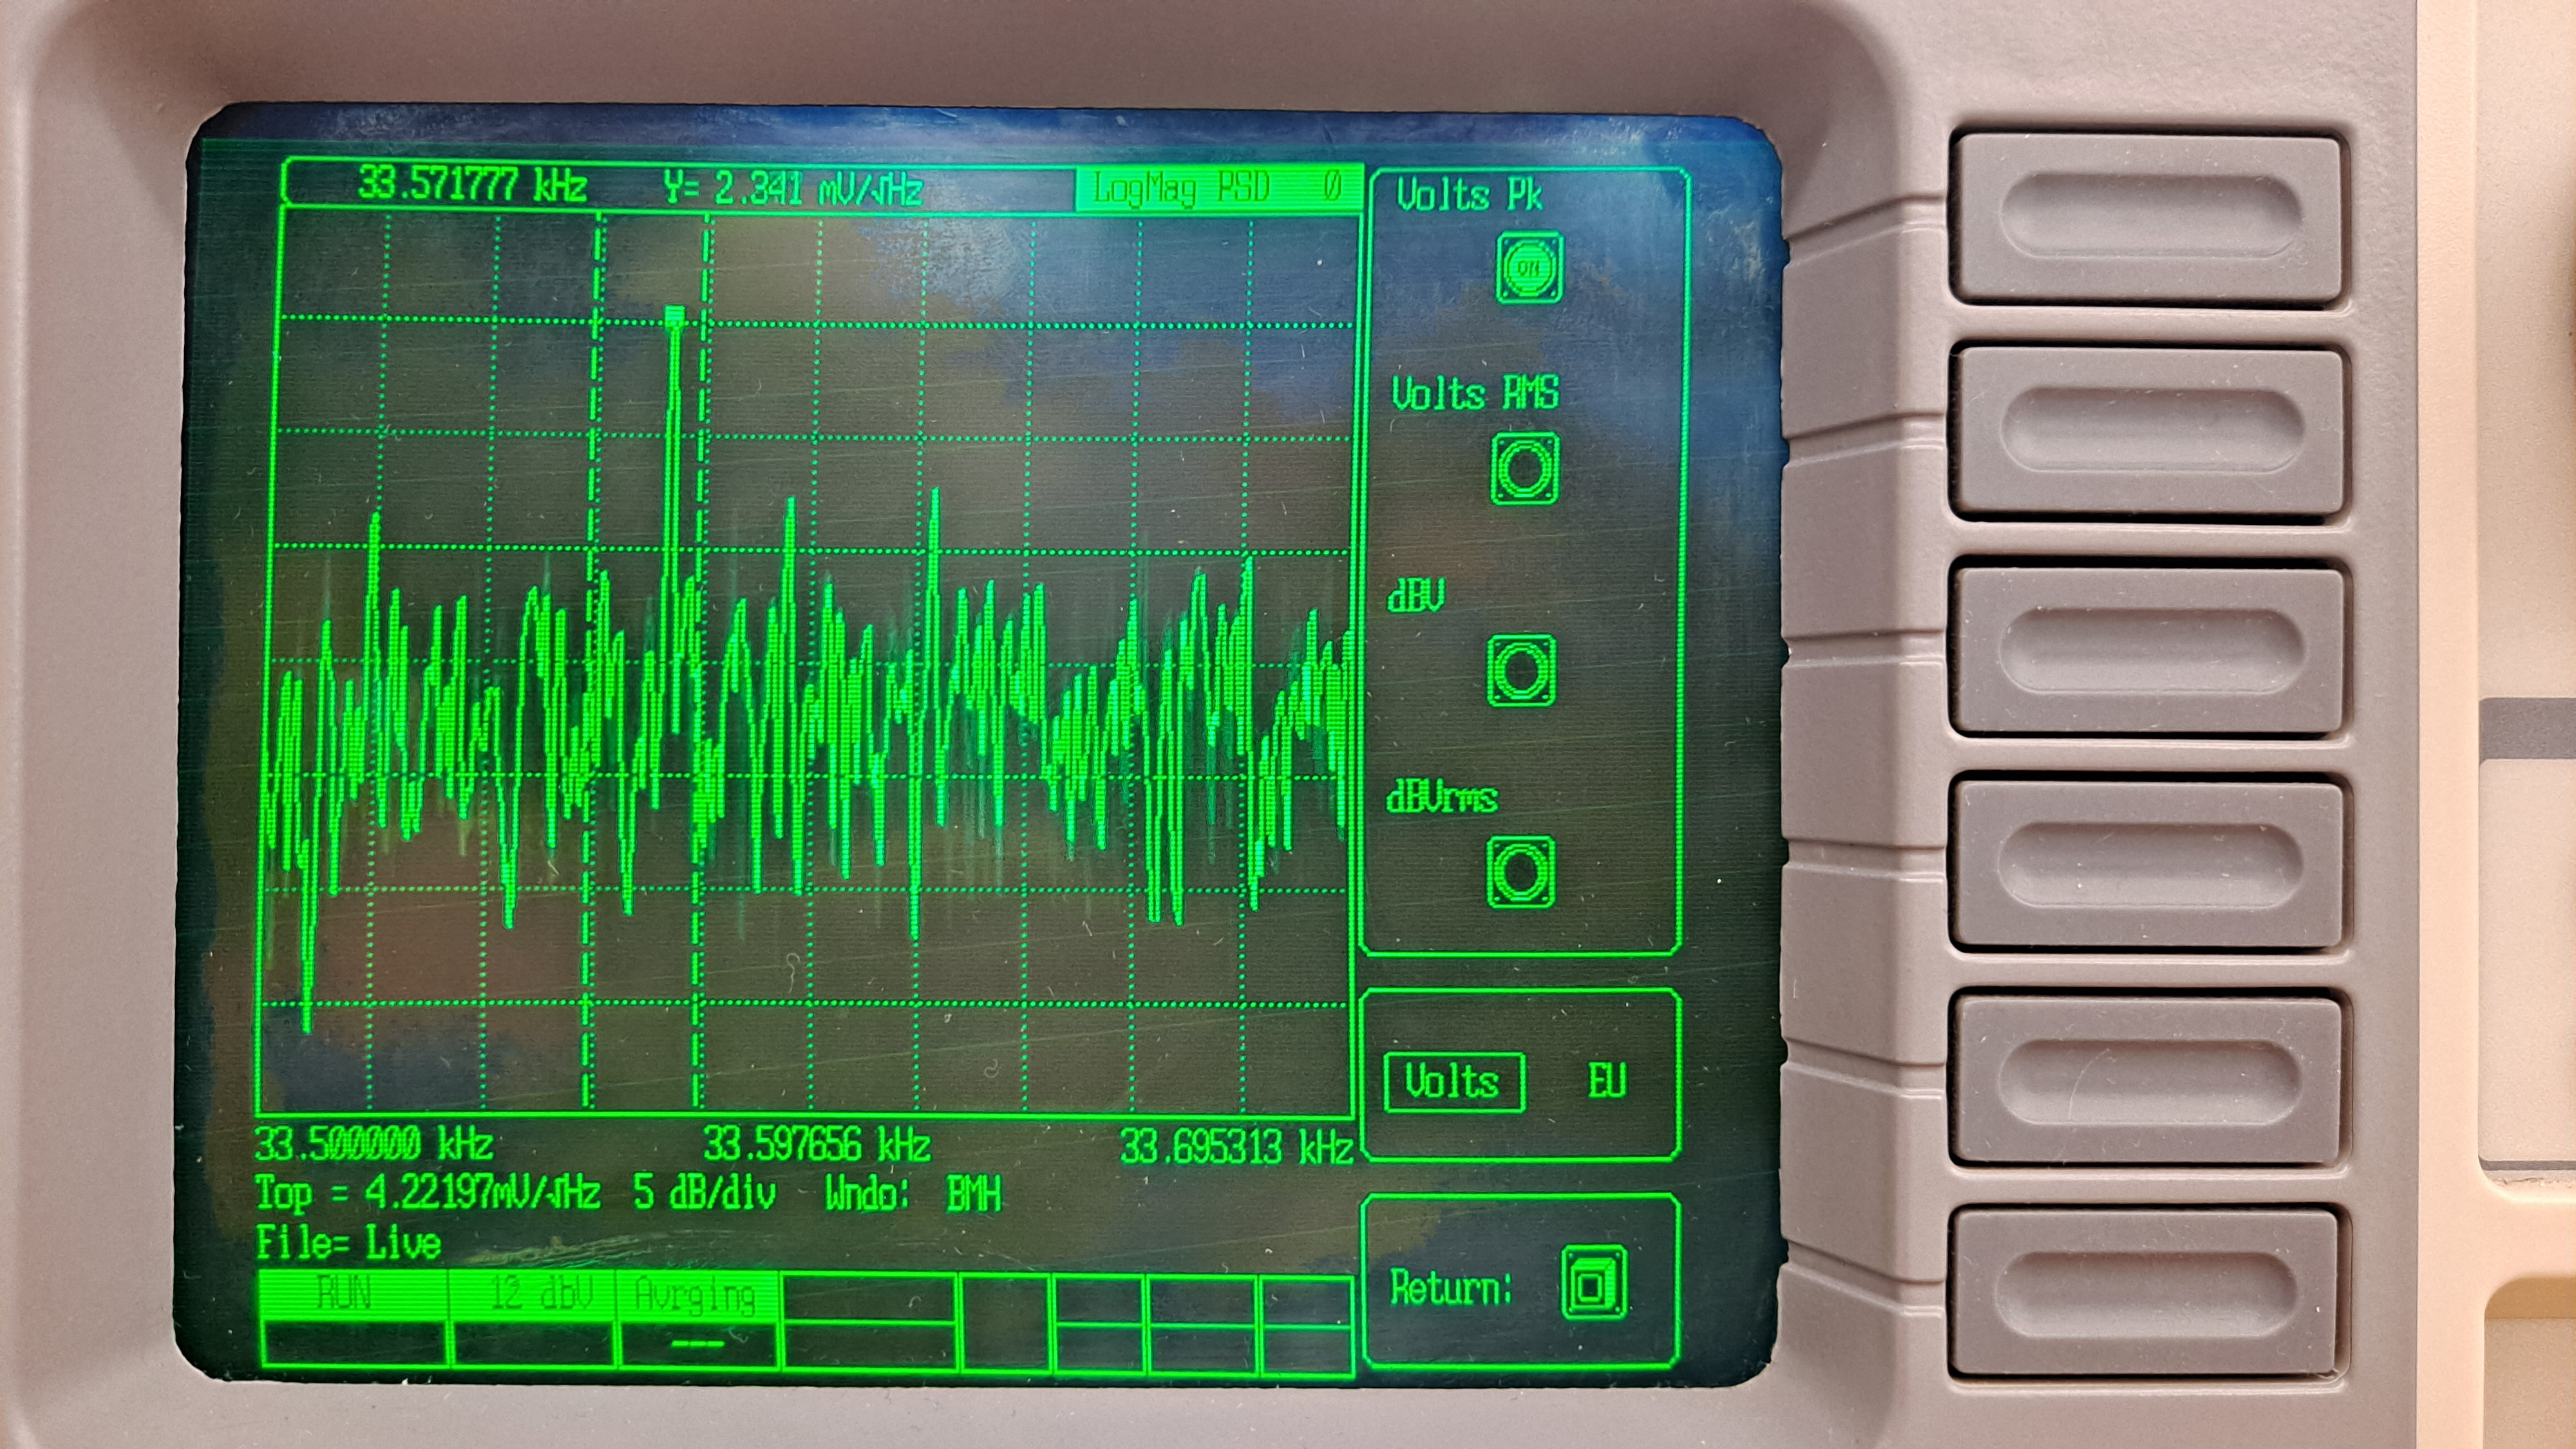
\includegraphics[width = 0.3\textwidth]{Signal C under Noise.jpg}
    \caption{\label{fig:2}Weak Signal under noise displayed in both the time and frequency domains.}
    \end{center}
\end{figure}

In this time display it is much harder to understand the nature of the underlying pure waveform.
A much weaker waveform has been superimposed upon stronger noise.
Despite this, in the frequency domain it is recoverable. 
This required more searching and decreasing the unit size of the display, effectively "zooming in".
Discovering an even weaker signal would require an even finer search, but would technically still be possible.
Theoretically there is no limit to how weak a signal can be identified.
This is due to the way the spectrum analyzer displays data and the nature of noise.
Noise, defined as being a  random process, sends power to each frequency with equal chance.
Therefore if one takes an average of noise over enough time, the averages should resolve to a flat uniform distribution in the frequency domain, as shown in Fig 3.
Any interesting signal should be easily visible over the line as its average will vary from this.
Practically speaking, the SSR770 takes its averages over a finite amount of time referred to as acquisition time.
Thus the process involved in identifying a weak signal among noise is presented as translating the signal to the frequency domain, taking sufficient averages, and using a fine enough span to visually spot it.

\begin{figure}[H]
\begin{center}
\includegraphics[width = 0.3\textwidth]{Averaged Noise.jpg}
\label{averagenoise}
\caption{Frequency domain of noise averaged over time.}
\end{center}
\end{figure}

Beyond just detection, the Fourier Transform can be useful in analyzing the properties of waveforms as well.
In AM radio, program content consists of a variable signal and the product of that and a pure carrier frequency creates an amplitude modulated signal containing program data.
The first image in Fig 4 shows an example we generated, with the full signal above and the carrier sinusoidal below.
This is a fairly interesting signal, however, just like in the previous case, we can only gain so much information from this.
Moving to the frequency domain, we can better see the properties of the signal, The central peak is the carrier wave and the sidebands demonstrate program content.
This allows us to better view the entire AM spectrum. If, for instance as there is in real applications, numerous radio stations all broadcasting in space, how would our devices tune to the one we desire without this methodology. 
Using Fourier Transformations and the frequency domain we can see each individual station and the program content is represented by the sidebands on either side. 

\begin{figure}[H]
\begin{center}
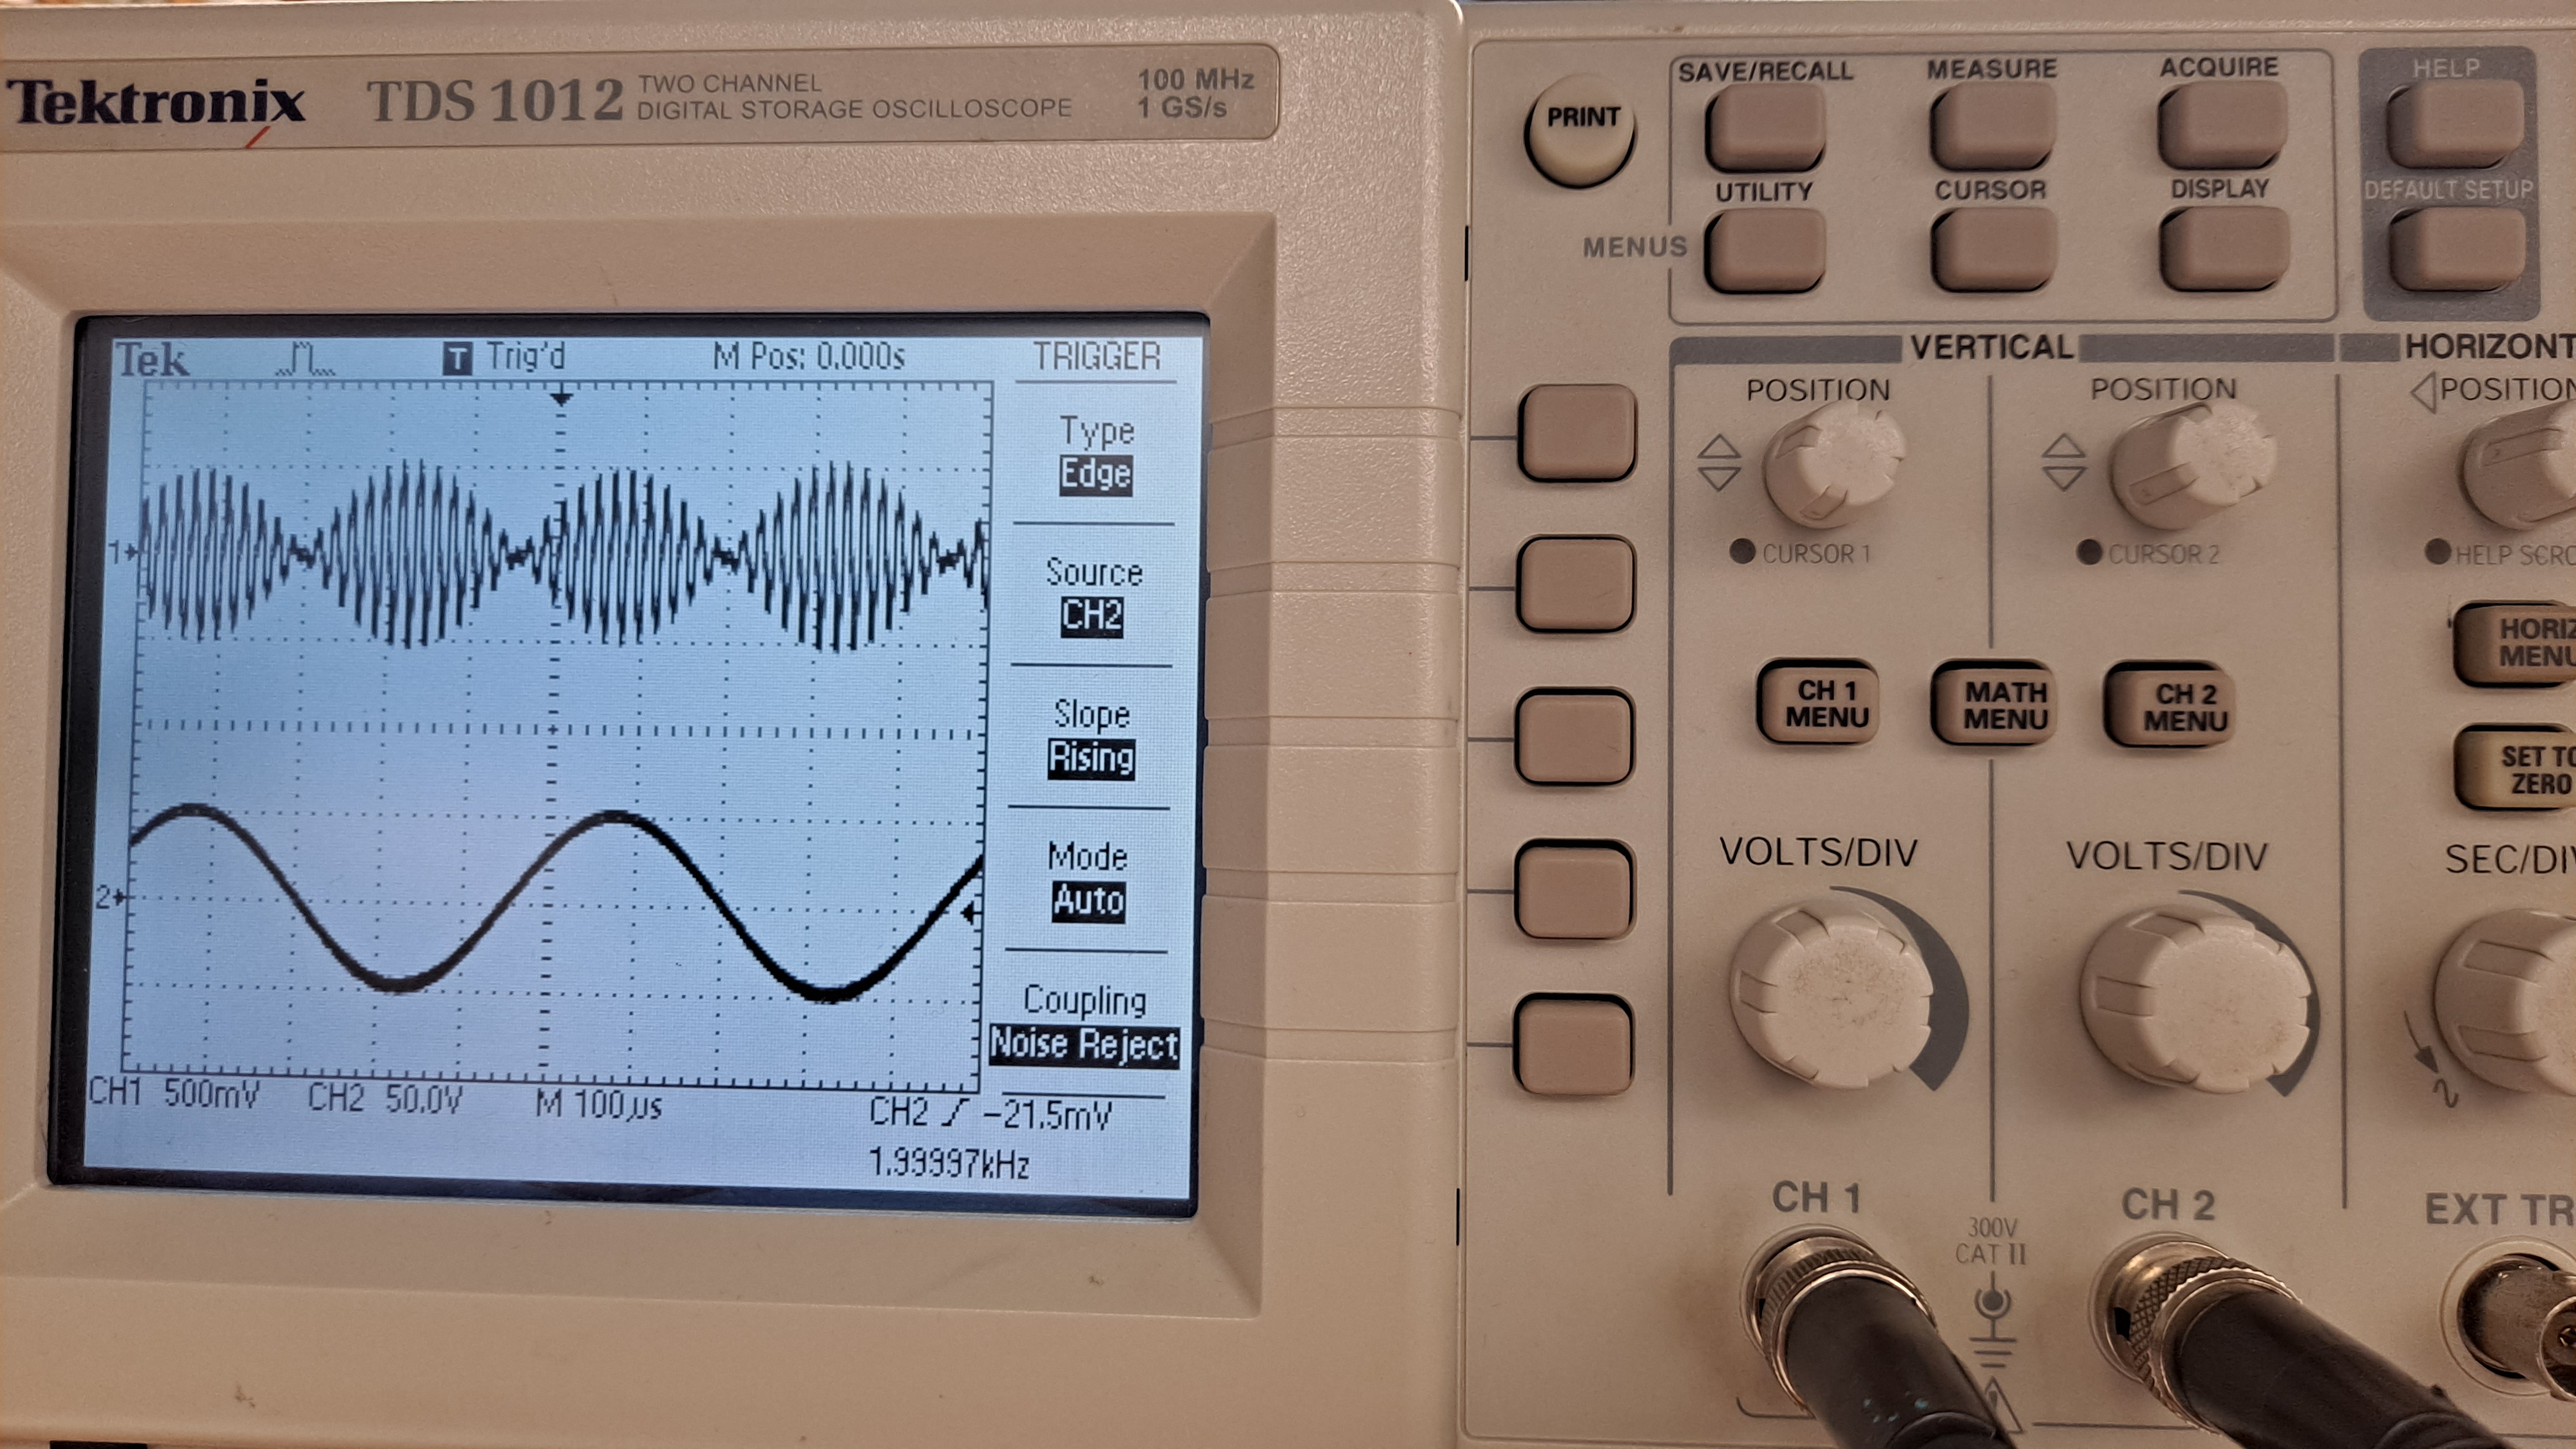
\includegraphics[width = 0.3\textwidth]{AM data, Time.jpg}
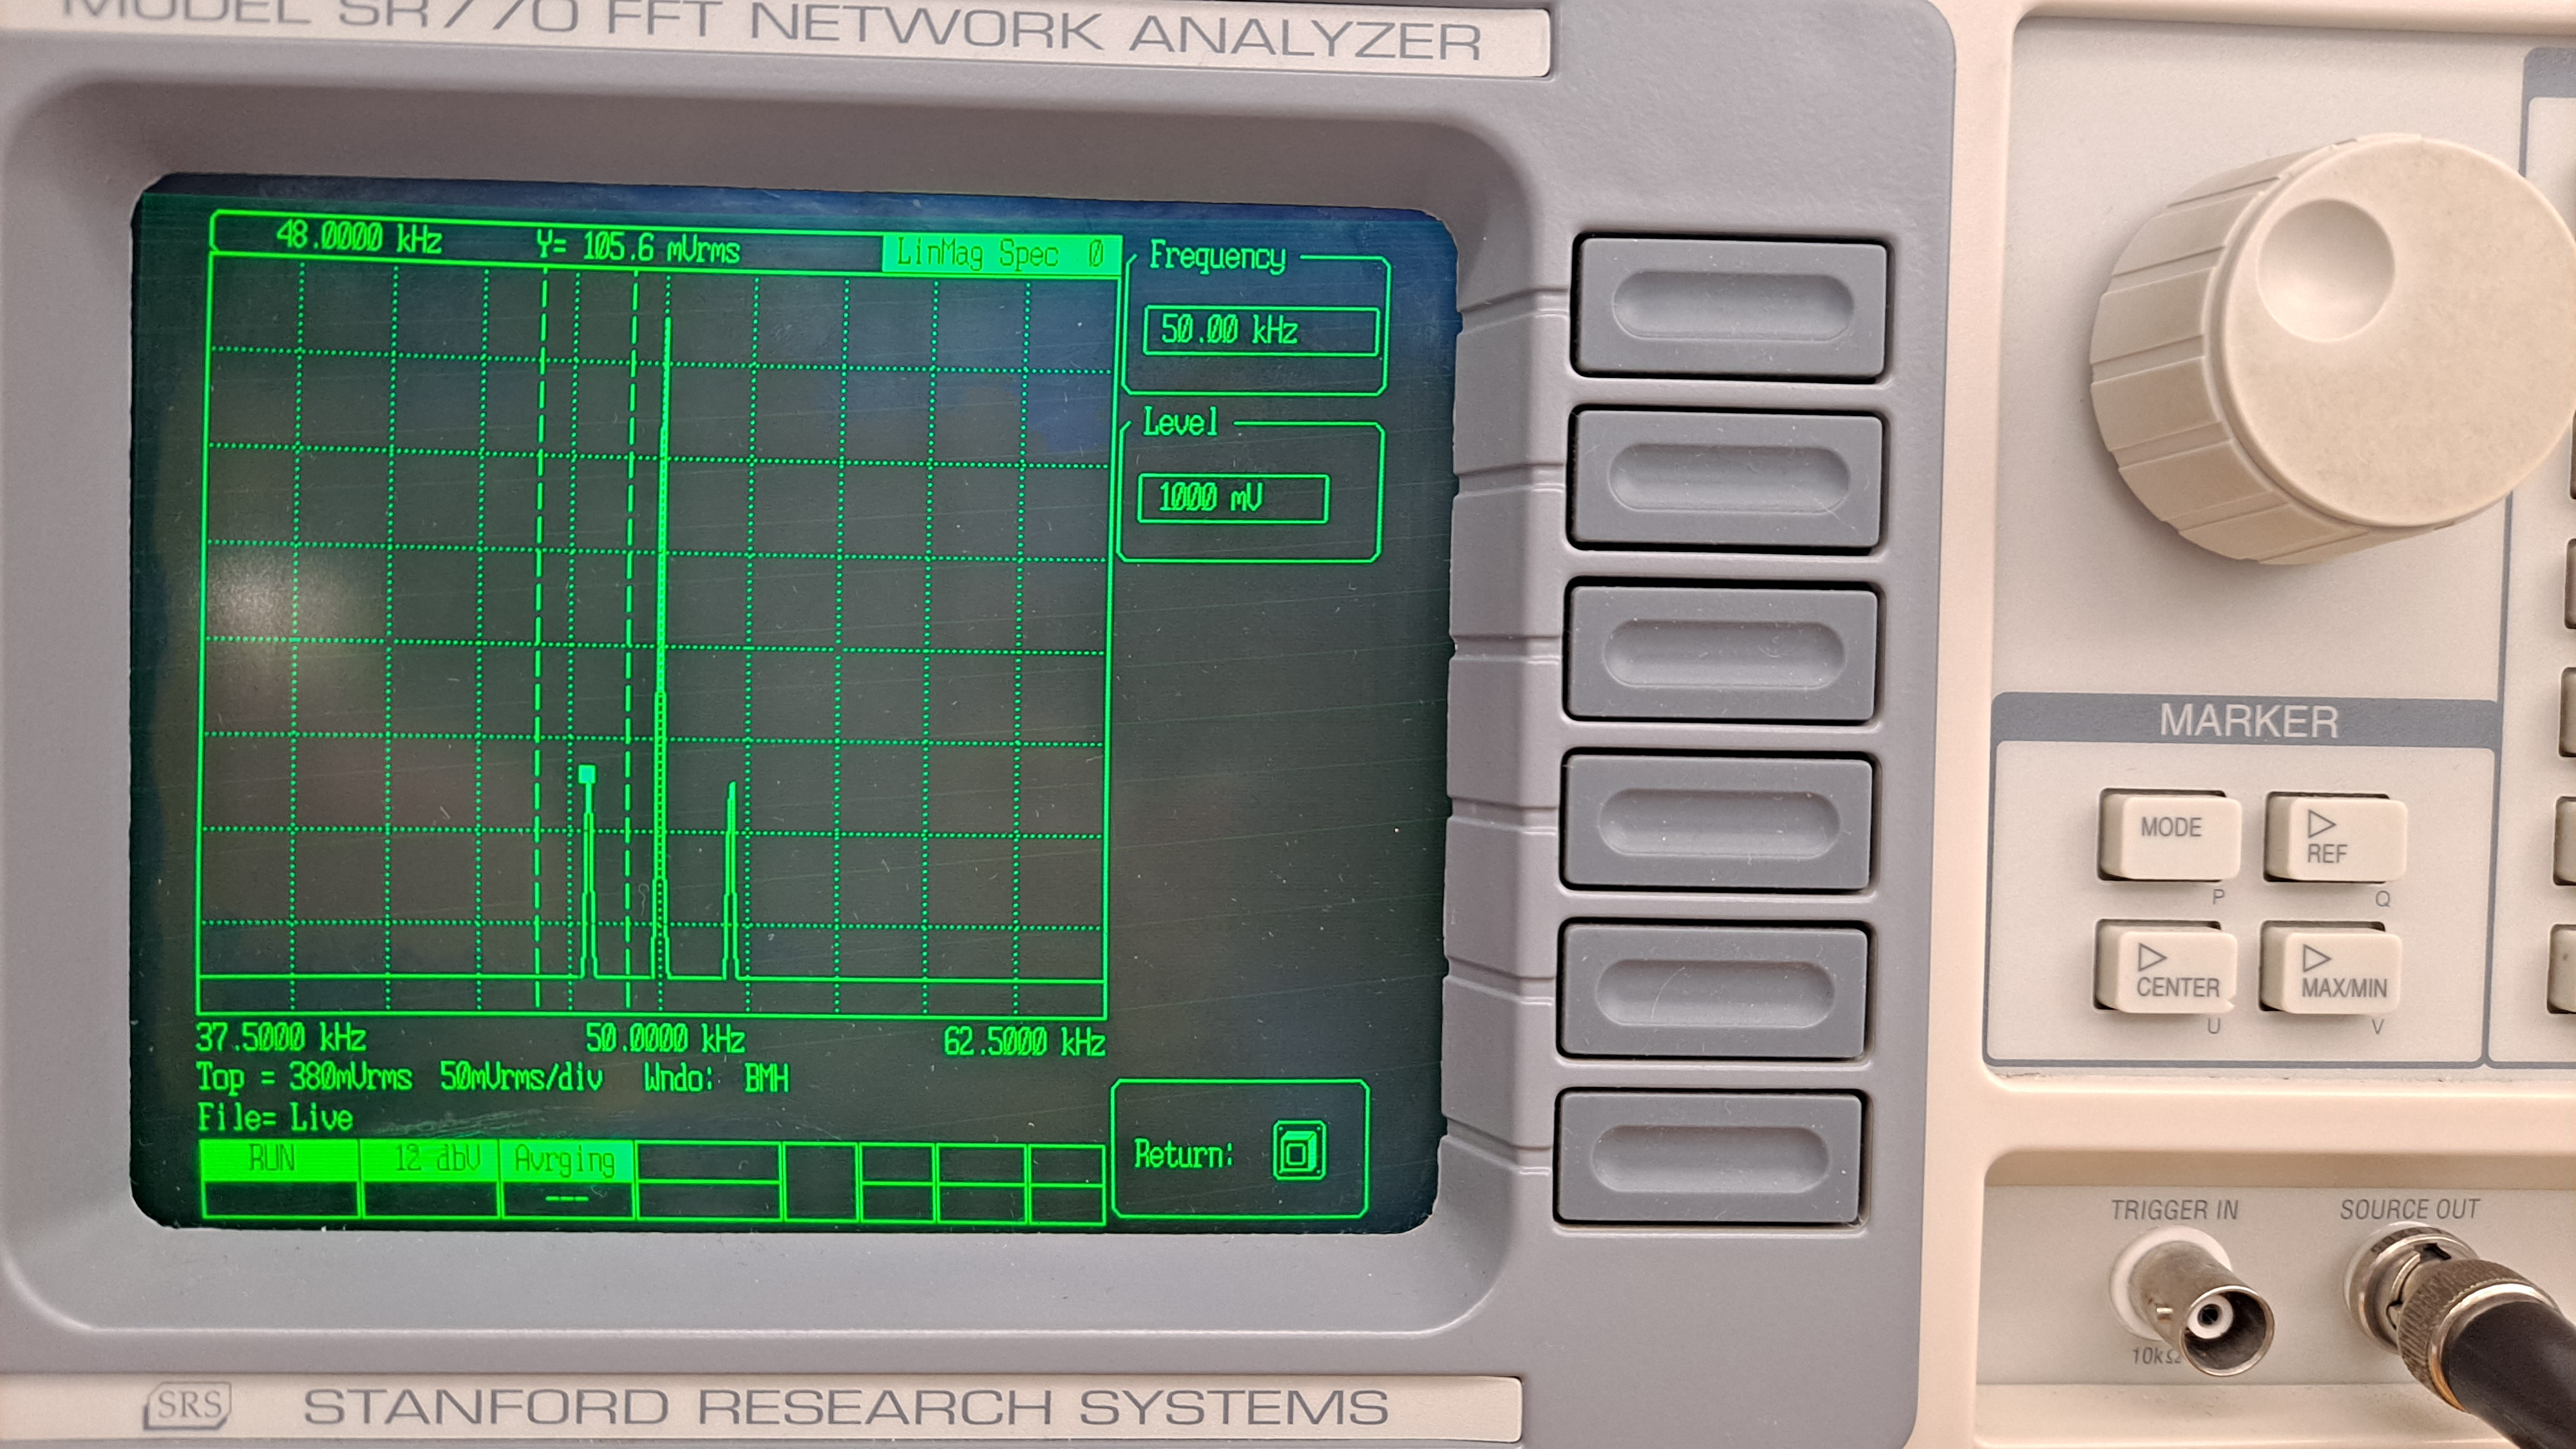
\includegraphics[width = 0.3\textwidth]{AM data, Freq.jpg}
\label{amsignal}
\caption{Data displayed for an Amplitude modulated signal in both domains.}
\end{center}
\end{figure}

Hopefully the varied nature of our application and analyses will motivate the reader that the Fourier Transformation is a useful lens for any signal analysis.
Viewing signals by their frequency domain should be, in the minds of these authors, a fundamental aspect of any data collection.
From radio telescope data to improved sound recognition in audio processing, Fourier demonstrates often unknown properties.
It can be applied to sensor data like in the magnetometer, but as we showed in the case of amplitude modulated wave forms, it can also reveal emergent properties in cases that may not have obviously called for its use.

\cite{Butz2015,James2011}
\bibliography{myrefs}

\end{document}
